% MS Thesis - Matthew Bohnsack

%\documentclass[twoside,botnum,fleqn,final]{unmeethesis}
\documentclass[botnum,fleqn,final]{unmeethesis}

% Set Title and Author
\newcommand{\mytitle}{Making Creative Commons More Effective\\with Usage Management}
\newcommand{\myauthor}{Matthew Paul Bohnsack}


% Font settings:
\usepackage[T1]{fontenc}
%\usepackage{mathpazo}
\usepackage{mathptmx}
\usepackage[scaled]{helvet}
\usepackage{courier}
\normalfont

% User microtype package to get some nicer font details
% http://www.ctan.org/tex-archive/macros/latex/contrib/microtype
\usepackage{microtype}

% Other packages
\usepackage{graphicx} % ability to include graphics
\usepackage[pdftex]{hyperref} % hyperrefs inside of PDF
\hypersetup{colorlinks,
            citecolor=black,
            filecolor=black,
            linkcolor=black,
            urlcolor=black,
            pdftitle={\mytitle},
            pdfauthor={\myauthor}}

% Use hyperref package to allow hyperlinks inside of the PDF document and PDF metadata
% http://en.wikibooks.org/wiki/LaTeX/Hyperlinks
\usepackage[pdftex]{hyperref}
\hypersetup{
    %bookmarks=true,          % show bookmarks bar?
    unicode=false,           % non-Latin characters in Acrobat’s bookmarks
    pdftoolbar=true,         % show Acrobat’s toolbar?
    pdfmenubar=true,         % show Acrobat’s menu?
    pdffitwindow=false,      % window fit to page when opened
    pdfstartview={FitH},     % fits the width of the page to the window
    pdftitle={\mytitle},     % title
    pdfauthor={\myauthor},   % author
    %pdfsubject={Subject},   % subject of the document
    %pdfcreator={Creator},   % creator of the document
    %pdfproducer={Producer}, % producer of the document
    %pdfkeywords={keyword1} {key2} {key3}, % list of keywords
    %pdfnewwindow=true,      % links in new window
    colorlinks=true,         % false: boxed links; true: colored links
    linkcolor=black,         % color of internal links
    citecolor=black,         % color of links to bibliography
    filecolor=black,         % color of file links
    urlcolor=blue            % color of external links
}

% We should look for graphics in these directories
\graphicspath{
{../resources/usecases/usecase1/}
{../resources/usecases/usecase2/}
{../resources/component-design/}
{../resources/implementation/}
{../resources/flickr/}
{../resources/cc/}
{../resources/pdfviewer/}
}

% http://www.gijsk.com/blog/2008/06/absence-citation-needed/
\usepackage{ifthen}
\let\oldcite=\cite
\renewcommand\cite[1]{\ifthenelse{\equal{#1}{NEEDED}}{[citation~needed]}{\oldcite{#1}}}

%%%%%%%%%%%%%%%%%%%%%%%%%%%%%%%%%%%%%%%%%%%%%%%%%%%%%%%%%%%%%%%%%%%%%%%%%%%%%%%%%%%%%%%%%
%%%%%%%%%%%%%%%%%%%%%%%%%%%%%%%%%%%%%%%%%%%%%%%%%%%%%%%%%%%%%%%%%%%%%%%%%%%%%%%%%%%%%%%%%
%%%%%%%%%%%%%%%%%%%%%%%%%%%%%%%%%%%%%%%%%%%%%%%%%%%%%%%%%%%%%%%%%%%%%%%%%%%%%%%%%%%%%%%%%

\begin{document}

\frontmatter

\title{\mytitle}
\author{\myauthor}

\degreesubject{M.S., Computer Engineering}

\degree{Master of Science \\ Computer Engineering}

\documenttype{Thesis}

\previousdegrees{A.S., Pre-Engineering, North Iowa Area Community College, 1994 \\
                 B.S., Electrical Engineering, Iowa State University, 1997}

%\date{September, \thisyear}
\date{\today}

\maketitle

\makecopyright

\begin{dedication}
   This thesis is dedicated my wife Elisa and our two daughters Evelyn and Katherine.
\end{dedication}

\begin{acknowledgments}
   \vspace{1.1in}
   I would like to thank my advisor, Professor Gregory Heileman, for his support.
\end{acknowledgments}

\maketitleabstract

\begin{abstract}
The Creative Commons provides legal and technical infrastructure that allows
intellectual property to be shared in terms that are more flexible than the
default ``all rights reserved''.  Under Creative Commons licenses, content can
be distributed widely online, but still controlled with specific,
well-understood common terms, such that authors reserve some rights.  More and
more content is being shared online under Creative Commons licenses.  As such,
it is very easy to create mash-ups or derivative works, based on many different
assets licensed under different Creative Commons licenses.  What's not so easy
is to pick a license compatible with all the different licenses inside of a
derivative work or to make sure all the licenses in a derivative work are
compatible with each other.

This paper looks at the conceptual and technical foundations of the Creative
Commons, takes a survey of how these things are commonly used on the Internet
today, and proposes an architecture, including usage management, that can be
used to make Creative Commons more effective.  An implementation of the proposed
architecture is presented along with a discussion on new functionality and future
work it could enable.
%\clearpage %(required for 1-page abstract)
\end{abstract}

\tableofcontents
\listoffigures
\listoftables

\begin{glossary}{UHR}
   \item[RDFa] Resource Description Framework -- in -- attributes
   \item[XDM] Extensible Metadata Platform
   \item[XML] eXtensible Markup Language
\end{glossary}

\mainmatter

%%%%%%%%%%%%%%%%%%%%%%%%%%%%%%%%%%%%%%%%%%%%%%%%%%%%%%%%%%%%%%%%%%%%%%%%%%%%%%%%%%%%%%%%%%
\chapter{\label{chapter:intro}Introduction}
%%%%%%%%%%%%%%%%%%%%%%%%%%%%%%%%%%%%%%%%%%%%%%%%%%%%%%%%%%%%%%%%%%%%%%%%%%%%%%%%%%%%%%%%%%

%%%%%%%%%%%%%%%%%%%%%%%%%%%%%%%%%%%%%%%%%%%%%%%%%%%%%%%%%%%%%%%%%%%%%%%%%%%%%%%%%%%%%%%%%%
\section{\label{section:intro:motivation}Motivation}
%%%%%%%%%%%%%%%%%%%%%%%%%%%%%%%%%%%%%%%%%%%%%%%%%%%%%%%%%%%%%%%%%%%%%%%%%%%%%%%%%%%%%%%%%%

%This is the introduction, and this is a example of a
%citation.\cite{McCarron:09:H} It's possible to do multiple citations at
%once.\cite{McCarron:09:H,Pemberton:08:RXS,Birbeck:08:RP,ccREL}

% http://wiki.creativecommons.org/Case_Studies/Flickr
Creative commons is being used more and more on the web.  For example, the
popular photo- and video-sharing site Flickr has published a case-study
claiming that they were hosting over 200 million CC licensed images as of
October 2011.\cite{NEEDED}  In March of 2010, Creative Commons published a
graph of the number of CC licensed images on Flickr.\cite{NEEDED}  This graph
showing growth from 2006 to 2010 is reproduced in
figure~\ref{fi:CC-growth-on-Flickr} on page~\pageref{fi:CC-growth-on-Flickr}.

% http://creativecommons.org/weblog/entry/20870
\begin{figure}[!htpb]
    \begin{center}
            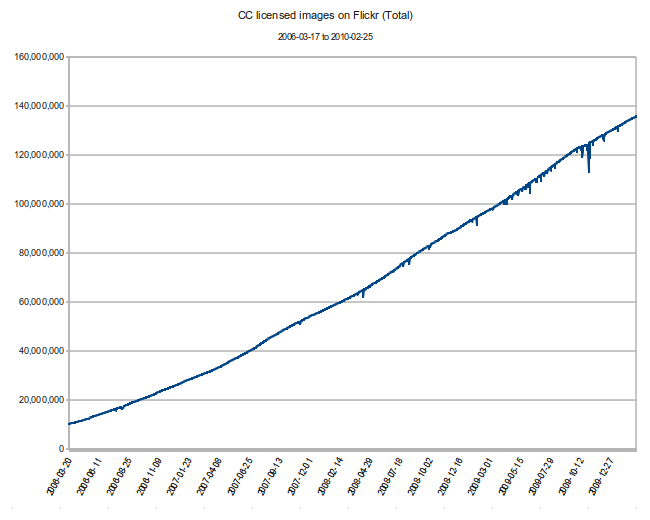
\includegraphics[width=1.0\textwidth]{cc-flickr-total-20100225.png}
    \end{center}
    \caption[CC licensed image on Flickr (Total)]{CC licensed images on Flickr (Total)}
    \label{fi:CC-growth-on-Flickr}
\end{figure}

This is an incredible number of images, and Flickr is not the only place that
CC licensed content can be found on the Internet.  A more detailed look at CC
content on the Internet is given in Section~\ref{section:intro:cconi}.

With all the images, video, text and other content that can be found on the web
under different CC licenses, it is very each for make a mash-up document
containing ``found content''.  However, it is not so easy to make sure you are
following all the rules when you create derivative works (mash-ups).  If you
combine dozens or even hundreds of assets together, each of which might have a
slightly different Creative Commons license, how can you ensure that your
intended use is 100\% compliant with all of the licensed content?  Further, if
an asset you want to use has a license incompatible with your intended use, is
there an easy way for you to acquire an alternative license that lets you use
the asset in the way you want to? 


%%%%%%%%%%%%%%%%%%%%%%%%%%%%%%%%%%%%%%%%%%%%%%%%%%%%%%%%%%%%%%%%%%%%%%%%%%%%%%%%%%%%%%%%%%
\section{\label{section:intro:cc}Creative Commons}
%%%%%%%%%%%%%%%%%%%%%%%%%%%%%%%%%%%%%%%%%%%%%%%%%%%%%%%%%%%%%%%%%%%%%%%%%%%%%%%%%%%%%%%%%%

\subsection{Overview}\label{section:intro:cc:overview}
%%%%%%%%%%%%%%%%%%%%%%%%%%%%%%%%%%%%%%%%%%%%%%%%%%%%%%%%%%%%%%%%%%%%%%%%%%%%%%%%%%%%%%%%%%

The Creative Commons is a nonprofit organization that provides free,
easy-to-use legal tools that provide a simple, standardized way to pre-clear
usage rights to creative works for copyright owners.  It gives copyright
holders an easy way to license their works in a way that leaves ``some rights
reserved'' as compared to the ``all rights reserved'' default.  By providing
these legal tools, the Creative Commons hopes to increase the amount of
creativity available ``in the commons''.  These licenses are not an alternative
to copyright.  Instead they apply on top of copyright, clarifying which rights
are extended to others and which rights are retained by the authors, under
their copyrights.

The Creative Commons provides detailed guidelines for annotating text, images,
audio, and video, to clearly specify how content is licensed, with a small
common set of relatively easy to understand licenses.  They also provide
guidelines for publishing via file sharing and social networking sites.  Some
support is provided for embedding license information as meta-data within
digital files.  The architecture presented in this paper makes extensive use of
the electronic embedding of license information in files.

It is important to understand a few other things about Creative Commons.
Firstly content licensed under Creative Commons licenses is not changeable or
revocable.  That is, once someone has received a copy of some CC-licensed
content, the work is perpetually licensed under the license it was received
under.  Secondly, view is always permissible under CC.  In other words, no CC
license prevents someone from viewing, reading, or listening to the CC-licensed
content.  Secondly, non-exclusive CC licenses are possible.  This means, for
example, that a particular piece of content may be licensed to the general
public in a way that is relatively restrictive, but if someone wanted a less
restrictive license, they could negotiate with the copyright holder for a
different license.

\subsection{License Types}\label{section:intro:cc:license types}
%%%%%%%%%%%%%%%%%%%%%%%%%%%%%%%%%%%%%%%%%%%%%%%%%%%%%%%%%%%%%%%%%%%%%%%%%%%%%%%%%%%%%%%%%%

Seven main license types are defined by Creative Commons:

\begin{enumerate}
  \item \emph{Public Domain}:

  This license doesn't put any restrictions on how others may remix, tweak, or
  build upon your work.

  \item \emph{Attribution}:

  This license lets others distribute, remix, tweak, and build upon your work,
  even commercially, as long as they credit you for the original creation. This
  is the most accommodating of the licenses offered.  It is recommended for
  maximum dissemination and use of licensed materials.

  \item \emph{Attribution, Share-Alike}:

  This license lets others remix, tweak, and build upon your work even for
  commercial purposes, as long as they credit you and license their new
  creations under the identical terms.  This license is often compared to free
  and open source software licenses.  All new works based on yours will carry
  the same license, so any derivatives will also allow commercial use.

  \item \emph{Attribution, No-Derivatives}:

  This license allows for redistribution, commercial and non-commercial, as
  long as it is passed along unchanged and in whole, with credit to you.

  \item \emph{Attribution, Non-Commercial}:

  This license lets others remix, tweak, and build upon your work
  non-commercially, and although their new works must also acknowledge you and be
  non-commercial, they don't have to license their derivative works on the same
  terms.

  \item \emph{Attribution, Non-Commercial, Share-Alike}:

  This license lets others remix, tweak, and build upon your work
  non-commercially, as long as they credit you and license their new creations
  under the identical terms.

  \item \emph{Attribution, Non-Commercial, No-Derivatives}:

  This license is the most restrictive of the licenses, only allowing others to
  download your works and share them with others as long as they credit you, but
  they can't change them in any way or use them commercially.
\end{enumerate}

All of the six non-Public Domain licenses can be made non-exclusive with
``CC+''\cite{NEEDED}.  This provides an explicit mechanism by which a
CC-licensed work can be marked up to express that different custom license
terms can be negotiated and how the author might be contacted to start such
negotiation.

\subsection{Creative Commons Rights Expression Language}\label{section:intro:cc:ccrel}
%%%%%%%%%%%%%%%%%%%%%%%%%%%%%%%%%%%%%%%%%%%%%%%%%%%%%%%%%%%%%%%%%%%%%%%%%%%%%%%%%%%%%%%%%%

blarg.


%%%%%%%%%%%%%%%%%%%%%%%%%%%%%%%%%%%%%%%%%%%%%%%%%%%%%%%%%%%%%%%%%%%%%%%%%%%%%%%%%%%%%%%%%%
\section{\label{section:intro:cconi}Creative Commons on the Internet Today}
%%%%%%%%%%%%%%%%%%%%%%%%%%%%%%%%%%%%%%%%%%%%%%%%%%%%%%%%%%%%%%%%%%%%%%%%%%%%%%%%%%%%%%%%%%

%%%%%%%%%%%%%%%%%%%%%%%%%%%%%%%%%%%%%%%%%%%%%%%%%%%%%%%%%%%%%%%%%%%%%%%%%%%%%%%%%%%%%%%%%%
\section{\label{section:intro:um}Usage Management}
%%%%%%%%%%%%%%%%%%%%%%%%%%%%%%%%%%%%%%%%%%%%%%%%%%%%%%%%%%%%%%%%%%%%%%%%%%%%%%%%%%%%%%%%%%

%%%%%%%%%%%%%%%%%%%%%%%%%%%%%%%%%%%%%%%%%%%%%%%%%%%%%%%%%%%%%%%%%%%%%%%%%%%%%%%%%%%%%%%%%%
\section{\label{section:intro:rw}Related Work}
%%%%%%%%%%%%%%%%%%%%%%%%%%%%%%%%%%%%%%%%%%%%%%%%%%%%%%%%%%%%%%%%%%%%%%%%%%%%%%%%%%%%%%%%%%

%%%%%%%%%%%%%%%%%%%%%%%%%%%%%%%%%%%%%%%%%%%%%%%%%%%%%%%%%%%%%%%%%%%%%%%%%%%%%%%%%%%%%%%%%%
\section{\label{section:intro:approach}Approach}
%%%%%%%%%%%%%%%%%%%%%%%%%%%%%%%%%%%%%%%%%%%%%%%%%%%%%%%%%%%%%%%%%%%%%%%%%%%%%%%%%%%%%%%%%%

%%%%%%%%%%%%%%%%%%%%%%%%%%%%%%%%%%%%%%%%%%%%%%%%%%%%%%%%%%%%%%%%%%%%%%%%%%%%%%%%%%%%%%%%%%
\chapter{\label{chapter:impl}Implementation}
%%%%%%%%%%%%%%%%%%%%%%%%%%%%%%%%%%%%%%%%%%%%%%%%%%%%%%%%%%%%%%%%%%%%%%%%%%%%%%%%%%%%%%%%%%

\begin{figure}[!htpb]
    \begin{center}
        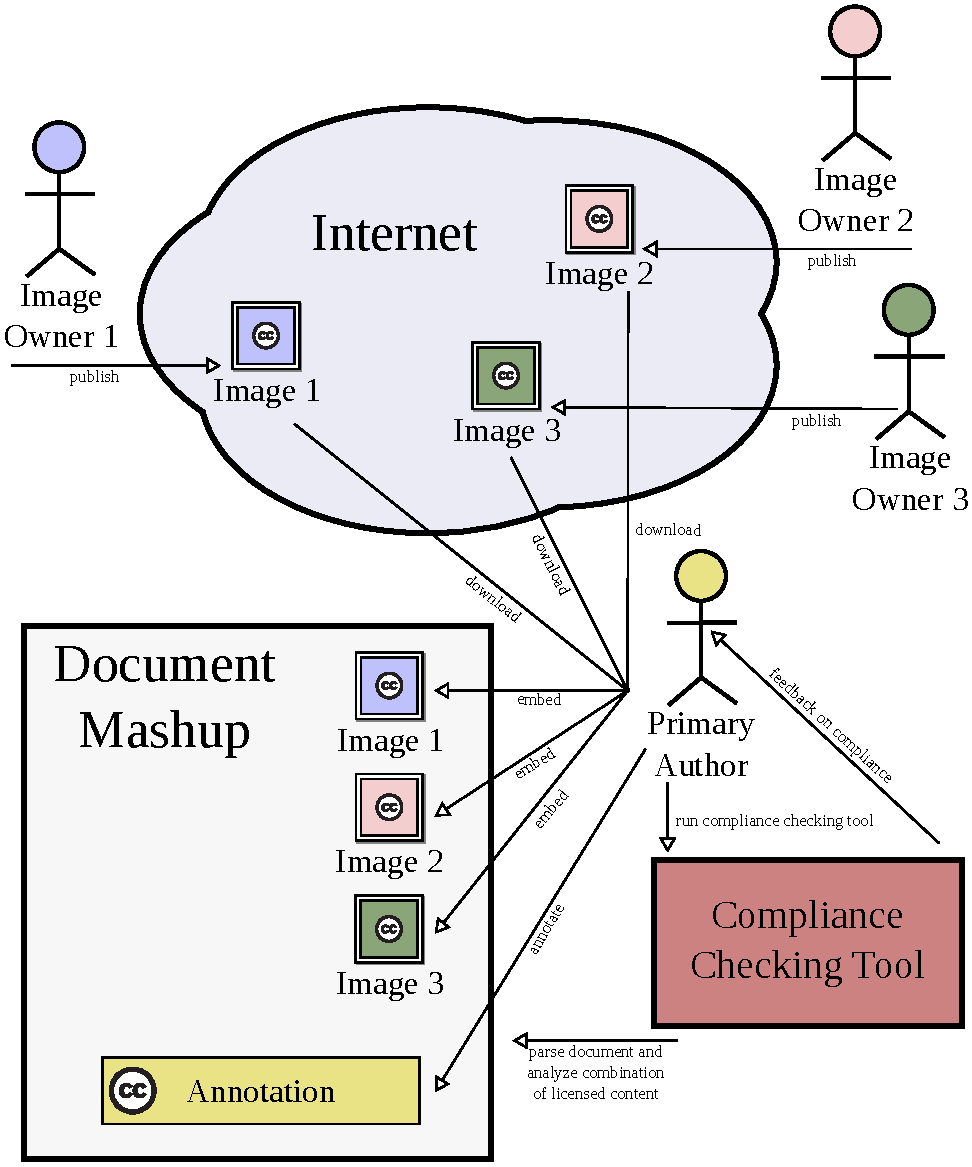
\includegraphics[width=1.0\textwidth]{usecase1-27.pdf}
    \end{center}
  \caption[Use case 1]{Use case 1.}
  \label{fi:usecase1}
\end{figure}

\begin{figure}[!htpb]
    \begin{center}
        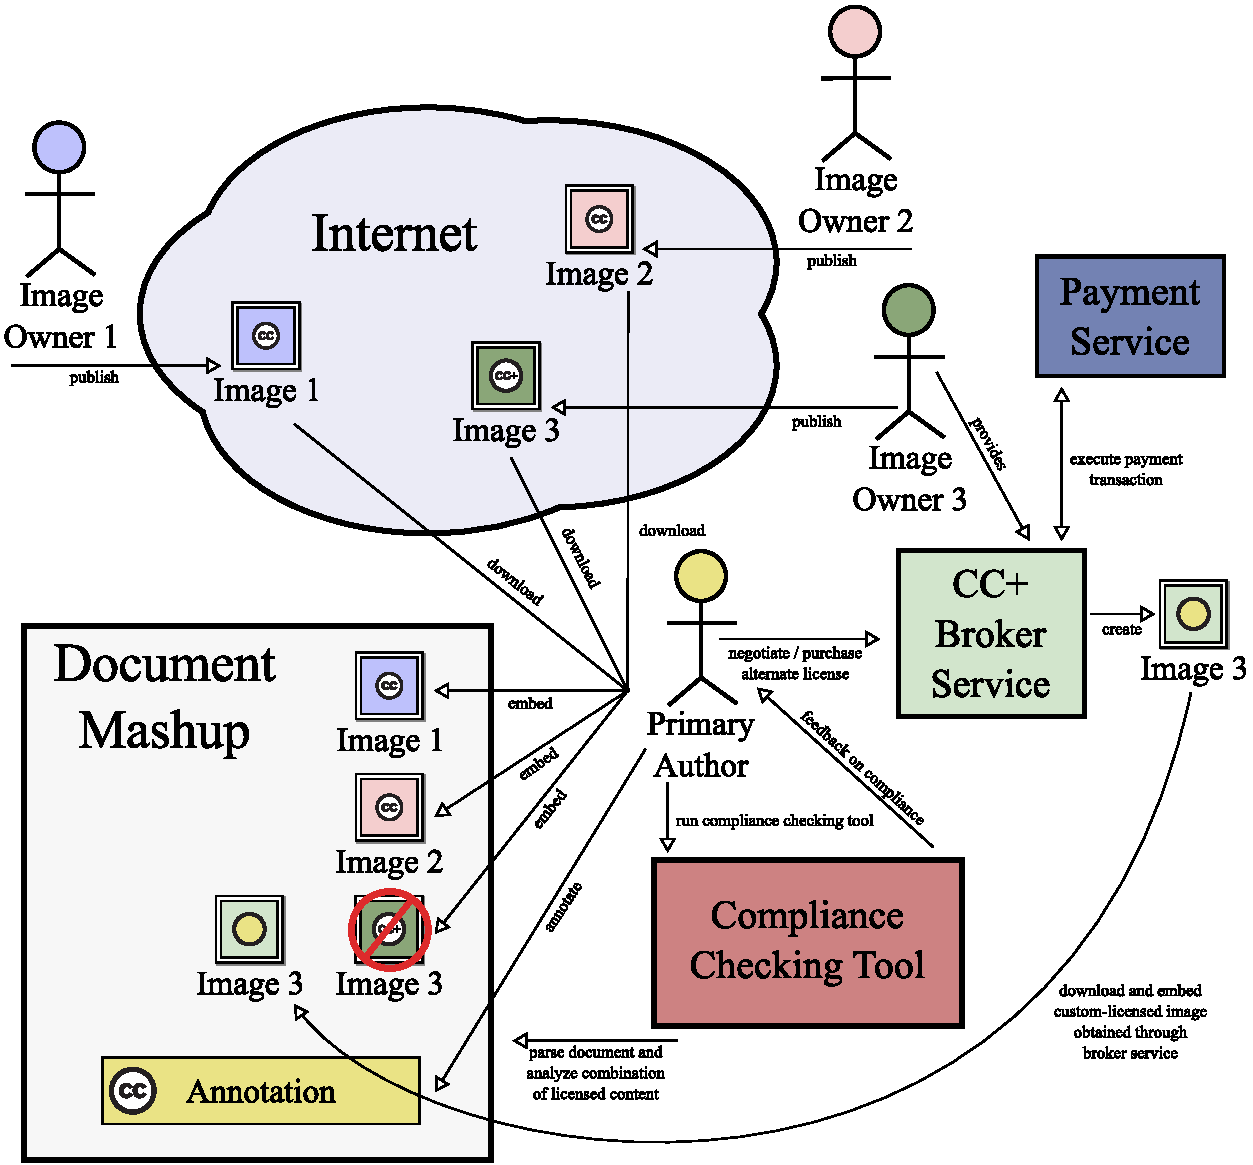
\includegraphics[width=1.0\textwidth]{usecase2-full2.pdf}
    \end{center}
  \caption[Use case 2]{Use case 2.}
  \label{fi:usecase2}
\end{figure}

\begin{figure}[!htpb]
    \begin{center}
            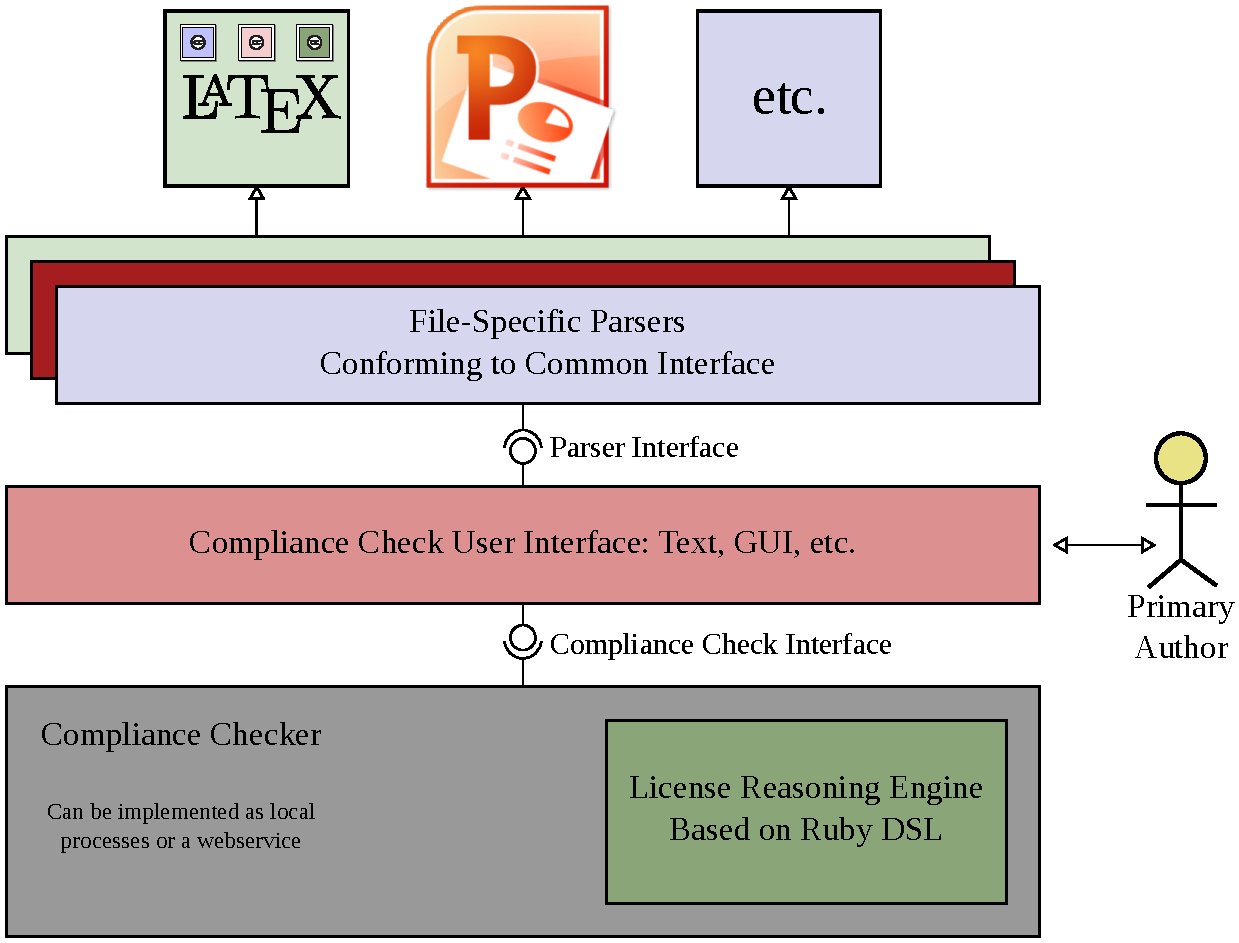
\includegraphics[width=1.0\textwidth]{compliance-checking-tool.pdf}
    \end{center}
    \caption[Compliance Checking Tool]{Compliance Checking Tool}
    \label{fi:complianceCheckingTool}
\end{figure}

\begin{figure}[!htpb]
    \begin{center}
            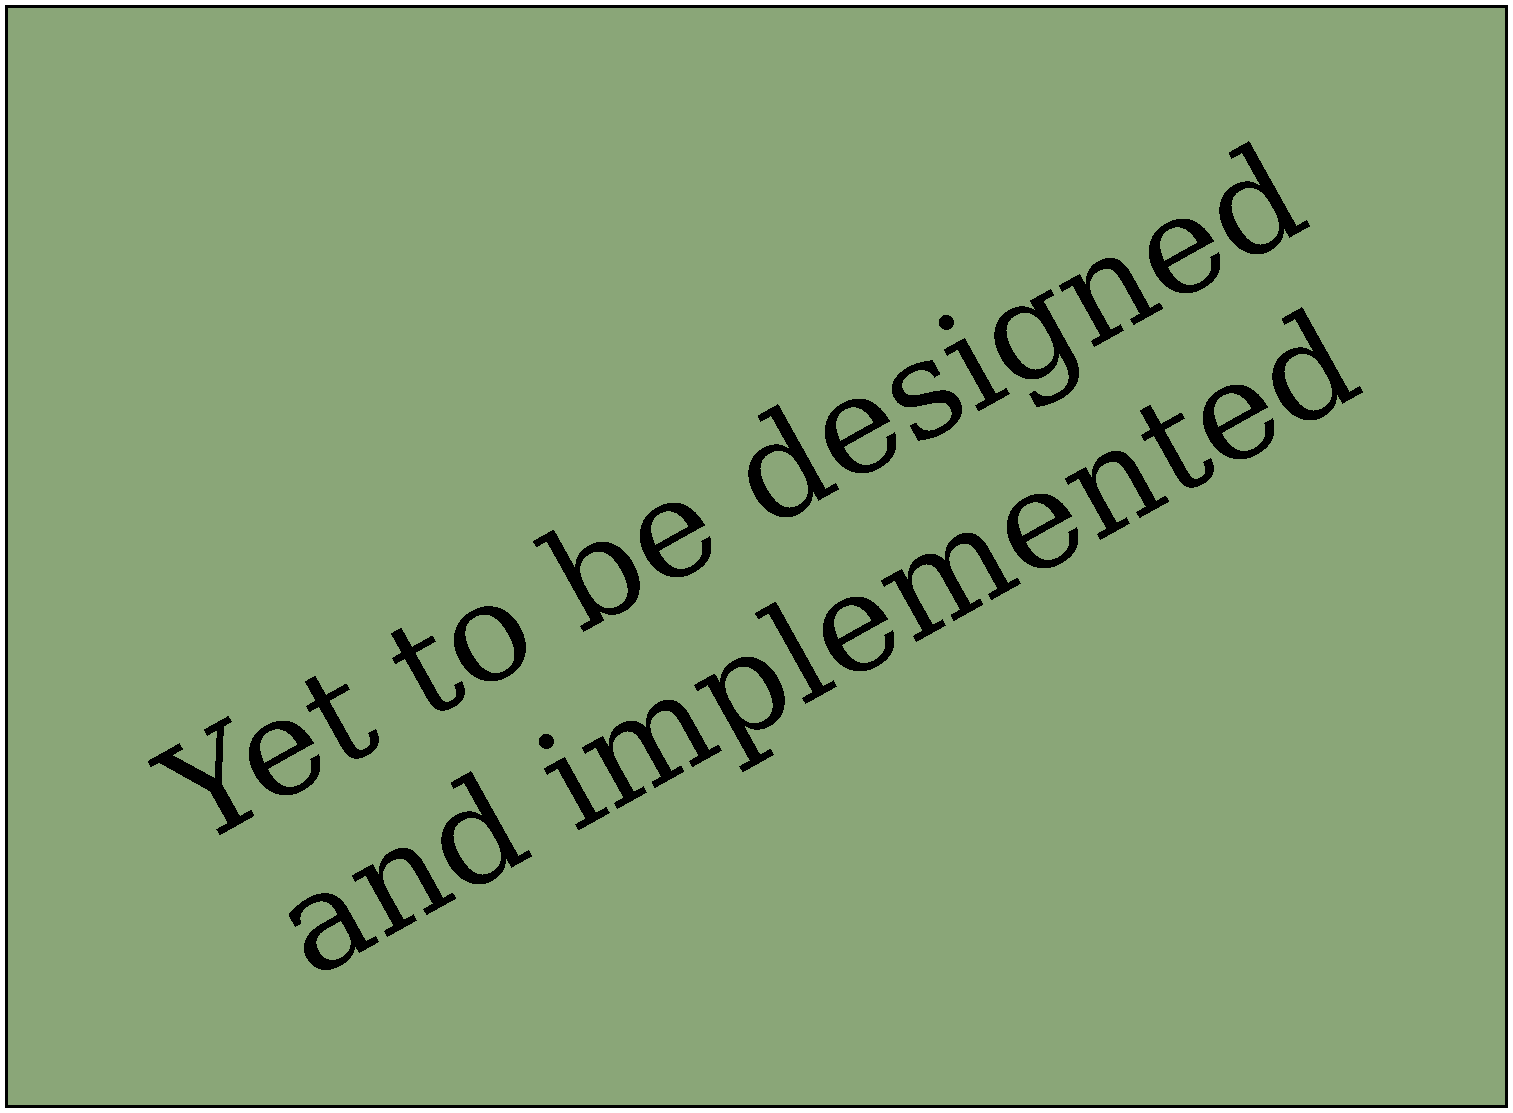
\includegraphics[width=1.0\textwidth]{todo.pdf}
    \end{center}
    \caption[License Reasoning Engine]{License Reasoning Engine}
    \label{fi:licenseReasoningEngine}
\end{figure}

\begin{figure}[!htpb]
    \begin{center}
            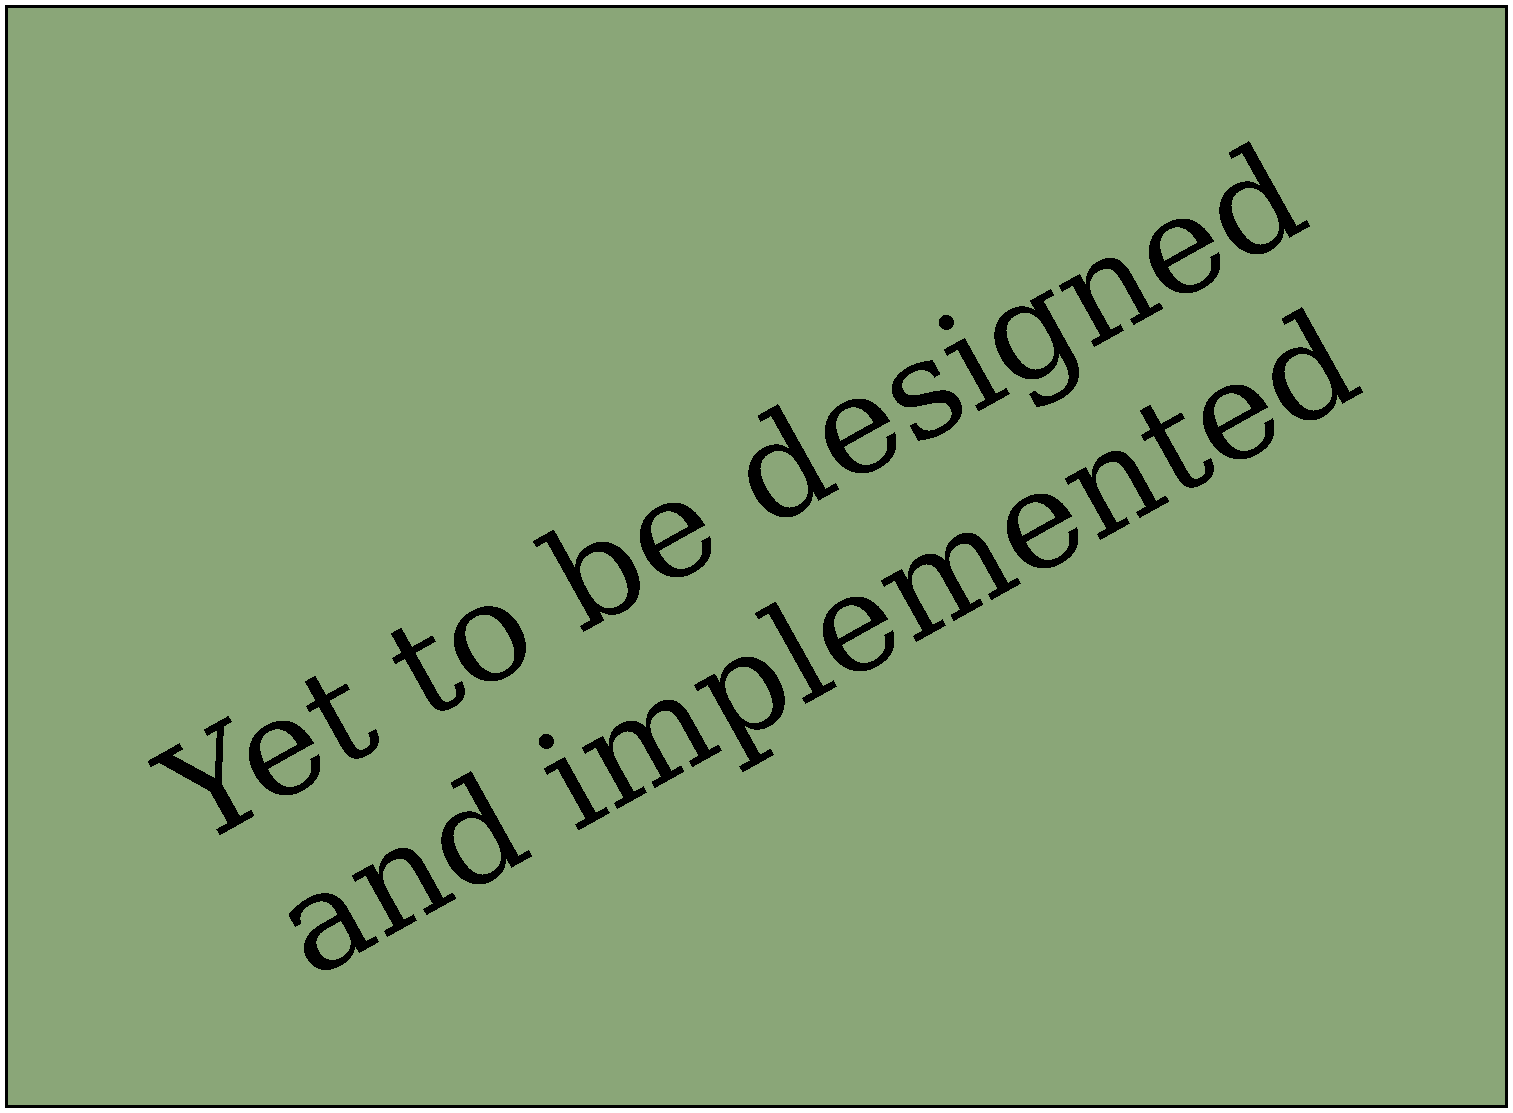
\includegraphics[width=1.0\textwidth]{todo.pdf}
    \end{center}
    \caption[CC+ Broker Service]{CC+ Broker Service}
    \label{fi:ccPlusBrokerService}
\end{figure}

%%%%%%%%%%%%%%%%%%%%%%%%%%%%%%%%%%%%%%%%%%%%%%%%%%%%%%%%%%%%%%%%%%%%%%%%%%%%%%%%%%%%%%%%%%
\chapter{\label{chapter:conc}Conclusions}
%%%%%%%%%%%%%%%%%%%%%%%%%%%%%%%%%%%%%%%%%%%%%%%%%%%%%%%%%%%%%%%%%%%%%%%%%%%%%%%%%%%%%%%%%%

Lorem ipsum dolor sit amet, consectetur adipiscing elit. Fusce vel orci massa.
In hac habitasse platea dictumst. Praesent non sem ut diam dignissim elementum.
Nulla in ligula non enim tristique dignissim. Pellentesque massa leo, ornare eu
rutrum quis, fringilla at odio. Aliquam leo mi, convallis et volutpat sed,
pellentesque at purus. Maecenas accumsan magna in ante mattis feugiat. Nam quis
nisi tellus. Pellentesque a lectus ipsum, eget suscipit ante. In hac habitasse
platea dictumst. Sed vulputate, arcu auctor sodales vehicula, nisi diam
dignissim dui, in mollis risus lectus id dolor. Sed ultricies tincidunt elit
sit amet egestas. Sed sed sodales purus. Proin scelerisque, diam at lacinia
tristique, metus nulla vehicula est, in blandit dui nibh non quam. Quisque
posuere porttitor mi in aliquam. Nullam eget pulvinar erat. Quisque ac velit ac
sapien porttitor euismod non et sem. Donec sodales, erat vitae vestibulum
eleifend, est nisl venenatis nibh, ac aliquet odio turpis scelerisque libero.
Sed sapien mauris, dapibus at luctus sed, scelerisque ut arcu.

Maecenas ac mauris urna. Praesent vehicula fringilla condimentum. Nam nec dolor
ac turpis accumsan scelerisque. Maecenas ut porttitor ipsum. Suspendisse
lobortis ligula ac metus adipiscing sollicitudin at vulputate lacus. Fusce
aliquet, libero quis tristique aliquet, nisl sem dapibus dui, mollis
sollicitudin diam metus at metus. Pellentesque ante ante, accumsan et mattis
ut, dictum eget libero. Etiam accumsan faucibus lectus, eu aliquet metus
tincidunt vitae. Sed nec lorem in tellus convallis porttitor nec et diam.
Praesent risus purus, venenatis vitae tincidunt ac, facilisis eget arcu.
Pellentesque sit amet nisi quis turpis laoreet venenatis eu in nunc.

Cras velit nibh, suscipit ac ultrices quis, laoreet nec elit. Proin varius, mi
non convallis sollicitudin, enim metus tristique lacus, non dignissim nibh nibh
vel turpis. Ut odio dui, vulputate sed commodo vel, venenatis ut ipsum. Lorem
ipsum dolor sit amet, consectetur adipiscing elit. Pellentesque est diam,
tristique ut facilisis eu, mattis pellentesque dolor. Nunc nulla dui, aliquet
eu semper at, consequat id odio. Suspendisse dignissim arcu non purus
vestibulum eu accumsan arcu vulputate. Cum sociis natoque penatibus et magnis
dis parturient montes, nascetur ridiculus mus. Cum sociis natoque penatibus et
magnis dis parturient montes, nascetur ridiculus mus. Cras vehicula massa id
sapien blandit tristique. Ut mattis dapibus malesuada. Integer rutrum, libero
et pellentesque venenatis, nisl ligula tempor diam, sit amet dapibus libero
arcu vitae sapien. Donec sagittis tincidunt elit non faucibus. Sed dapibus
augue a nulla ultrices aliquet fermentum odio consectetur. Sed volutpat ornare
porta. Curabitur dapibus nulla vel orci tempus at dignissim ante adipiscing.
Aliquam congue cursus semper. Cras nulla libero, porta ac ultrices nec,
consectetur sed justo. Donec sed augue mauris, vitae adipiscing eros.

Maecenas non velit sem, non mollis mi. Integer ut enim enim. Curabitur sed est
at tellus porttitor placerat. Maecenas ultrices turpis nec tortor interdum
convallis vitae et est. Nullam vestibulum elit et nisl mattis adipiscing.
Phasellus eget varius odio. Praesent ac metus at libero vestibulum luctus id
eget nisl. Praesent posuere massa eu urna blandit ut consequat justo pharetra.
Nunc faucibus enim a enim commodo dapibus. Mauris rhoncus eros nunc. Donec
feugiat urna ac quam elementum quis hendrerit sapien dignissim. Vestibulum
porta turpis ac lacus vestibulum ut consequat ipsum bibendum. Praesent pretium
eros sit amet mauris faucibus vitae ultrices nunc adipiscing. Fusce leo lectus,
consequat tincidunt aliquam vel, aliquet a ligula.

Quisque eget condimentum mauris. Nam quis purus eget justo venenatis vehicula
nec id velit. Curabitur a quam ipsum, luctus gravida urna. Integer tristique
risus et lectus dictum ac ultricies nulla pretium. Ut sit amet viverra diam.
Praesent ac nisl quis nibh bibendum ullamcorper. Nullam pharetra risus sit amet
tortor convallis euismod accumsan sit amet quam. Duis fermentum aliquet
suscipit. Praesent in sem eros, porta gravida quam. Sed elementum magna
fringilla leo fringilla semper ornare mauris pulvinar. In vel eleifend mauris.
Pellentesque neque tortor, euismod ut vestibulum rutrum, gravida sed sem. Lorem
ipsum dolor sit amet, consectetur adipiscing elit. Nunc tincidunt augue ac
tellus adipiscing fringilla. Suspendisse ac dolor orci. Praesent dictum dolor
quis lorem sollicitudin tempus. Nunc dictum pretium nunc, ac egestas velit
imperdiet eget. Curabitur nec mi massa, sit amet vestibulum libero.

%%%%%%%%%%%%%%%%%%%%%%%%%%%%%%%%%%%%%%%%%%%%%%%%%%%%%%%%%%%%%%%%%%%%%%%%%%%%%%%%%%%%%%%%%%
\chapter{\label{chapter:fw}Future Work}
%%%%%%%%%%%%%%%%%%%%%%%%%%%%%%%%%%%%%%%%%%%%%%%%%%%%%%%%%%%%%%%%%%%%%%%%%%%%%%%%%%%%%%%%%%

Lorem ipsum dolor sit amet, consectetur adipiscing elit. Fusce vel orci massa.
In hac habitasse platea dictumst. Praesent non sem ut diam dignissim elementum.
Nulla in ligula non enim tristique dignissim. Pellentesque massa leo, ornare eu
rutrum quis, fringilla at odio. Aliquam leo mi, convallis et volutpat sed,
pellentesque at purus. Maecenas accumsan magna in ante mattis feugiat. Nam quis
nisi tellus. Pellentesque a lectus ipsum, eget suscipit ante. In hac habitasse
platea dictumst. Sed vulputate, arcu auctor sodales vehicula, nisi diam
dignissim dui, in mollis risus lectus id dolor. Sed ultricies tincidunt elit
sit amet egestas. Sed sed sodales purus. Proin scelerisque, diam at lacinia
tristique, metus nulla vehicula est, in blandit dui nibh non quam. Quisque
posuere porttitor mi in aliquam. Nullam eget pulvinar erat. Quisque ac velit ac
sapien porttitor euismod non et sem. Donec sodales, erat vitae vestibulum
eleifend, est nisl venenatis nibh, ac aliquet odio turpis scelerisque libero.
Sed sapien mauris, dapibus at luctus sed, scelerisque ut arcu.

Maecenas ac mauris urna. Praesent vehicula fringilla condimentum. Nam nec dolor
ac turpis accumsan scelerisque. Maecenas ut porttitor ipsum. Suspendisse
lobortis ligula ac metus adipiscing sollicitudin at vulputate lacus. Fusce
aliquet, libero quis tristique aliquet, nisl sem dapibus dui, mollis
sollicitudin diam metus at metus. Pellentesque ante ante, accumsan et mattis
ut, dictum eget libero. Etiam accumsan faucibus lectus, eu aliquet metus
tincidunt vitae. Sed nec lorem in tellus convallis porttitor nec et diam.
Praesent risus purus, venenatis vitae tincidunt ac, facilisis eget arcu.
Pellentesque sit amet nisi quis turpis laoreet venenatis eu in nunc.

Cras velit nibh, suscipit ac ultrices quis, laoreet nec elit. Proin varius, mi
non convallis sollicitudin, enim metus tristique lacus, non dignissim nibh nibh
vel turpis. Ut odio dui, vulputate sed commodo vel, venenatis ut ipsum. Lorem
ipsum dolor sit amet, consectetur adipiscing elit. Pellentesque est diam,
tristique ut facilisis eu, mattis pellentesque dolor. Nunc nulla dui, aliquet
eu semper at, consequat id odio. Suspendisse dignissim arcu non purus
vestibulum eu accumsan arcu vulputate. Cum sociis natoque penatibus et magnis
dis parturient montes, nascetur ridiculus mus. Cum sociis natoque penatibus et
magnis dis parturient montes, nascetur ridiculus mus. Cras vehicula massa id
sapien blandit tristique. Ut mattis dapibus malesuada. Integer rutrum, libero
et pellentesque venenatis, nisl ligula tempor diam, sit amet dapibus libero
arcu vitae sapien. Donec sagittis tincidunt elit non faucibus. Sed dapibus
augue a nulla ultrices aliquet fermentum odio consectetur. Sed volutpat ornare
porta. Curabitur dapibus nulla vel orci tempus at dignissim ante adipiscing.
Aliquam congue cursus semper. Cras nulla libero, porta ac ultrices nec,
consectetur sed justo. Donec sed augue mauris, vitae adipiscing eros.

%\chapter*{Appendices}

%\addcontentsline{toc}{chapter}{Appendices}
 % Next lines duplicated from .toc file and used to create mini
 % "Appendix Table of Contents," if desired:
   %\contentsline {chapter}{\numberline {A}Proving the biggie}{4}
   %\contentsline {chapter}{\numberline {B}Derivation of somthing else}{5}
 % End mini table of contents

%\appendix
%\chapter{Proving the biggie}
%   For proving $E=MC^2$, I refer the reader to many of grandpa's famous books on this subject.
%\chapter{Derivation of somthing else}
%   To derive $A = \pi r^2$, simply not that a circle is really a square without corners.  QED.

%\bibliographystyle{AMS}
\bibliographystyle{plain}
\bibliography{ref}

\end{document}
